\documentclass{article}
\usepackage[margin=1.3in]{geometry}
\usepackage{amssymb}
\usepackage{amsmath}
\usepackage{syntax}
\usepackage{xspace}
\usepackage{graphicx}
\usepackage{subcaption}
\usepackage{array}

\usepackage[T1]{fontenc}
\usepackage{lmodern}

\usepackage{pdfpages}

\usepackage[backend=bibtex8]{biblatex}

\bibliography{bibliography}

\usepackage{todonotes}

%all used by listings
\usepackage{listings}
\usepackage{xcolor}   % for \textcolor
%\usepackage{graphicx}
\usepackage{amssymb}
\lstset{
  breaklines=true,
  frame=tblr,
  postbreak=\mbox{\textcolor{red}{$\hookrightarrow$}\space},
  basicstyle=\ttfamily\scriptsize,
  commentstyle=\color{gray}\ttfamily,
  keywordstyle=\color{blue}\ttfamily
}

\usepackage{color}
\definecolor{lightgray}{rgb}{.9,.9,.9}
\definecolor{darkgray}{rgb}{.4,.4,.4}
\definecolor{purple}{rgb}{0.65, 0.12, 0.82}
\lstdefinelanguage{TypeScript}{
  keywords={break, case, catch, class,constructor, continue, debugger, default, delete, do, else,export, false, finally, for, function, if,implements, in, instanceof, new, null, return, switch,static, this, throw, true, try, typeof, var, void, while, with},
  morecomment=[l]{//},
  morecomment=[s]{/*}{*/},
  morestring=[b]',
  morestring=[b]",
  ndkeywords={class, export, boolean, throw, implements, import, this},
  keywordstyle=\color{blue}\bfseries,
  ndkeywordstyle=\color{darkgray}\bfseries,
  identifierstyle=\color{black},
  commentstyle=\color{purple}\ttfamily,
  stringstyle=\color{red}\ttfamily,
  sensitive=true
}

%End of used by listings



\begin{document}

%New commands for listing requirements
\newcommand{\RSetup}[0]{R1\xspace}
\newcommand{\RCustom}[0]{R2\xspace}
\newcommand{\RLightweight}[0]{R3\xspace}
\newcommand{\RIntuitive}[0]{R4\xspace}
\newcommand{\RFamiliarity}{R5\xspace}

%\newcommand{\todo}[1]{==TODO: #1 ==}


%\include{requirements}
\section*{Abstract}
\todo{}

\section{Introduction}
\subsection{Relevant Background}
Before discussing my project's specific goals and outlining my contributions, I will discuss, at a high level, the topics which this project pertains too.
\subsubsection{Domain Specific Languages}

\todo{Complete}
\subsubsection{Language Workbenches}
\todo{Complete}
\subsubsection{Projectional Editing}
\todo{Complete}
\subsection{Project Aims and Motivation}

\subsubsection{Problem To Address}\label{problem}

This project seeks to address the following problem. An often cited use case for DSLs is to enable domain experts to write code to solve issues within their domain in an efficient manner \todo{Reference here}. However, these experts are not necessarily experienced at writing code.  \todo{reference here the finance case from blog or book} To those without prior experience, traditional, textually based programming can seem alienating and complex, \todo{ see if source exists} making it difficult for language designers to target such users.
\\
\\
Projectionally editing code is one potential solution to this problem, allowing the user to interact with the code in a way which is intuitive and familiar. Although a projectionally based language workbench, MPS\cite{mps}, exists, it is geared towards projections which look primarily like traditional textual code, which we are trying to prevent in the case of interacting with users as described above. There is also a significant feature disparity between it and it's parser-based rivals (unfortunately this is common between language workbenches). One feature it is notably lacking is the ability to generate a web-based editor application.

\subsubsection{Project Goal}
This project's goal was to extend an existing language workbench, or to create a new one, with the capability of generating a web-based, projectional editor for a DSL specified in that workbench. 

\subsubsection{Motivation}
Currently, the ability to automatically generate a projectional editor as a web application for an arbitrary language specification, does not exist in any major language workbench. However, I believe this functionality would be useful for the following reasons:
\begin{itemize}
\item Web editing is particularly useful for DSLs, speeding up the deployment of newly created languages by reducing the need to share/install IDEs or plugins after every iteration of the language (which likely change frequently in their infancy). 
\item Projectional editors can reduce, and in some cases completely eliminate, the time required by a user to learn the syntax of a language. This is useful for DSLs where the language is likely only used for a small part of a project and will not be commonly known.
\item Crucially, the combination of these features is ideal for addressing the problem laid out in section \ref{problem}. A web editor ensures that there is no need to install or use an IDE for the language, which are often notoriously complex. A projectional editor may then allow them to interact with the language in an environment they are used to, perhaps by filling in forms and tables or drawing a diagram.  
\end{itemize} 
As further affirmation to the potential usefulness of this feature, we look at the existing sprotty framework being developed by Typefox\cite{sprotty}, a prominent group of contributers to the open-source language workbench Xtext. Sprotty aims to provide graphical views of textual code by integrating with language servers produced by the language workbench Xtext. A web based projectional editor could not only offer this view, but also allow the user to interact with this view directly to modify their code, which is clearly far more powerful. 

\subsubsection{Requirements}\label{requirements}
To be able to evaluate the final implementation I here set out the necessary requirements we should meet in order to fulfil our goal: 

\begin{itemize}
\item{\textbf{R1: Quick to setup} - It should be as quick and easy as possible for a language designer to create a projectional editor. Just as language workbenches automatically create eclipse plugins or standalone IDEs with little or no input from the user, so should our editors be generated automatically, so the designer need only worry about language specific concerns.}
\item{\textbf{R2: Customisable} - Despite the above point the editor should be highly customisable if desired. We should aim to deliver as much as possible to the language designer "for free" but shouldn't prevent them from customising or modifying as required for their application. }
\item{\textbf{R3: Lightweight Editor} - By default the resultant web application should be as lightweight as possible, although always a neccesary concern with web applications this is especially important here as whereas often it is assumed that developer's machines will be powerful, here we are also specifically targeting less technically inclined users who are likely on less competent machines}
\item{\textbf{R4: Intuitive Editor} - As before we are specifically targeting less technically inclined users, and so any default interface should be as intuitive as possible for non-developers.}
\item{\textbf{R5: Familiarity} - The process for creating a new language and accompanying editor should be as familiar to the language designer as possible. They should have to learn as few new technologies/languages/processes as possible.}
\end{itemize}

\subsection{Contributions}

In order to achieve the project's goal my contributions can be split into 3 key areas:

\begin{enumerate}
\item The specification of a server-side web API to allow a client application to edit an arbitrary programming language projectionally.
\item The development of a DSL for specifying projections of an arbitrary programming language's abstract syntax tree, which may easily be displayed and interacted with within a web browser.
\item The extension of the language workbench Xtext such that, given a language specification of a DSL, it can automatically generate a web application capable of using (1) to projectionally edit the language using projections specified with (2).
\end{enumerate}


\subsection{Organisation} 
\todo{TODO}
\section{Technical Background}
\todo{TODO}
\subsection{MPS}
\todo{TODO}
\subsection{Xtext}
\todo{TODO}
\subsection{Abstract Syntax tree}
\todo{TODO}
\subsection{Eclipse}
\todo{TODO}
\subsection{EMF}
\todo{TODO}
\subsection{MWE2}
\todo{TODO}
%
%
%
%Overview
%
%
%
%
\section{Automatic Generation Of Projectional Web Editors In XText}
In this section I will discuss my extension to the language workbench XText. I begin by giving a quick overview of the extension before moving onto to it's use from a user's perspective, and then covering the more interesting sections of it's design in detail. This includes the API implemented by the generated language server, and the projection specification DSL. I focus throughout on design decisions that have been made as a result of the requirements outlined in section \ref{requirements}. 


\subsection{Overview}

The final tool takes the form of an extension to the language workbench Xtext, which is itself an Eclipse\cite{eclipse} plugin. A designer can use this extended plugin to create a projectional editor by first specifying a language grammar using XText's existing grammar language, and then generating projectional editor artefacts. These consist of:
\begin{itemize}
\item A back-end Java servlet which is capable of interacting with a client application using the HTTP API discussed later in section \ref{api}. \todo{Check ref working}
\item A Java servlet container to host these servlets
\item An empty \emph{.editor} file in which a language designer can use the language discussed in section \ref{EditorLanguage} \todo{Check ref working} to specify custom projections for their nodes if desired.  
\end{itemize}
%
I have also created a default client web application using the Angular application platform\cite{angular}, which can be hosted by the generated language server and then used by the language's end user to interact with the server to display and edit the designed language through the specified custom projections. 

\subsection{Benefits of integration with Xtext}\label{integrationWithXtext}
Before continuing with the design, I discuss the rationale behind the integration with Xtext. The decision was primarily made as by extending an existing language workbench I didn't have to concern myself with rewriting all the core functionality of a workbench from scratch (e.g. the abilities to specify a grammar, building a parser etc.) and instead could focus on the implementation of projectional editing. By extending an existing popular workbench we are working towards our \RFamiliarity requirement of familiarity, and Xtext was a prime candidate for a number of reasons:
\begin{itemize}
\item{It is open-source and so easy to modify}
\item{It is one of the most popular language workbenches available and so has much support available}
\item{It internally uses EMF\cite{emf}, which allows for bidirectional transformations between, in effect, our abstract syntax tree and it's textual representation. This is useful for a number of reasons which I will later discuss\todo{If I have reference section}}
\end{itemize}

\subsection{The Generation Process}
I will now discuss the process of generating a projectional language server from a specified language using my plugin. To meet our \RSetup requirement the generation process was designed to be as simple as possible, so that a language designer can concentrate their efforts on the DSL specification. The process was also designed to be as close as possible to the process of setting up a textual web editor in XText, to satisfy our familiarity \RFamiliarity requirement.
\\
\\
The language designer first creates an Xtext project as normal, using the Eclipse new project wizard as shown in figures \ref{fig:newProjectWiz},
\begin{figure}[t!]
  \centering
  \begin{subfigure}[b]{0.45\linewidth}
    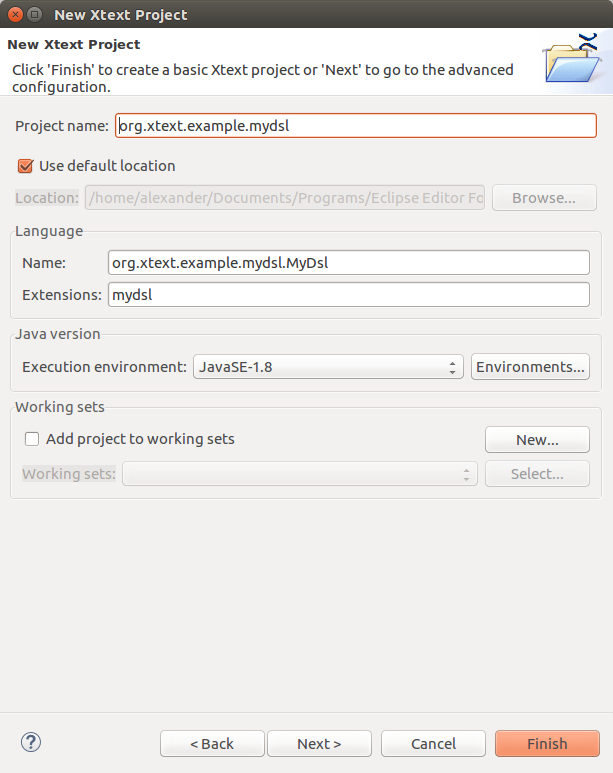
\includegraphics[width=\linewidth]{./Screenshots/newXtextProject.png}
    \caption{page 1}
  \end{subfigure}
  \begin{subfigure}[b]{0.45\linewidth}
    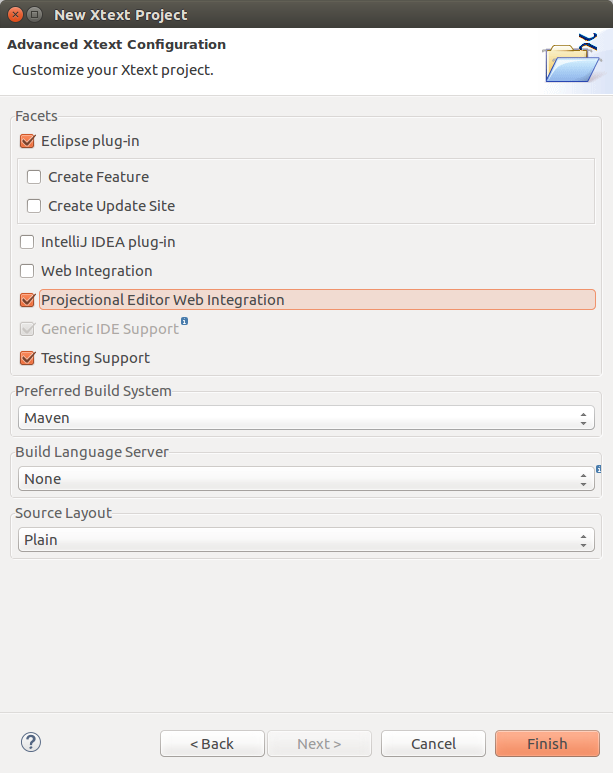
\includegraphics[width=\linewidth]{./Screenshots/newXtextProjectPage2.png}
    \caption{page 2}
  \end{subfigure}
  \caption{The modified "new xtext project" wizard}
  \label{fig:newProjectWiz}
\end{figure}
selecting the "Projectional Editor Web Integration" facet which has been added to the wizard next to the existing option for creating a textual web editor.
\\
\\
This creates an Xtext language project, shown in figure
\begin{figure}[h!]
  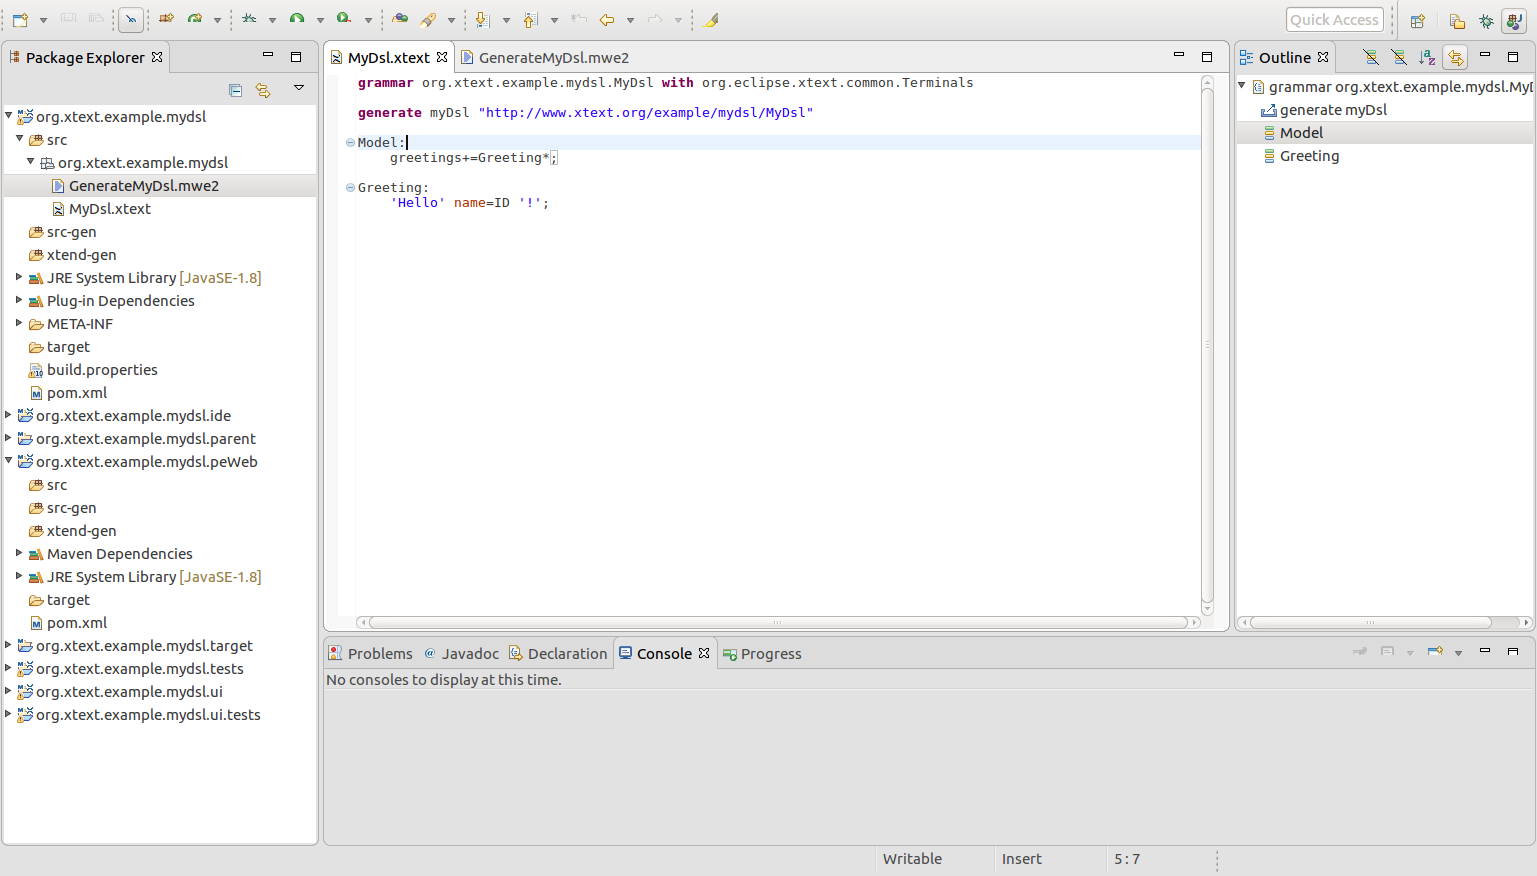
\includegraphics[width=\linewidth]{./Screenshots/newProjectScreen.png}
  \caption{A new xtext project with an empty peWeb project}
  \label{fig:newProjectScreen}
\end{figure} \ref{fig:newProjectScreen}, with a \emph{.xtext} file to specify the DSL's grammar and a \emph{.MWE2} file to describe the generation of the selected facets as usual. A number of empty projects are also created which will contain the files generated by the grammar definition. Notice the \emph{org.xtext.example.mydsl.peWeb} project which has been created and populated with a maven \emph{.pom} file which will be responsible for dependency management and has automatically been configured with the dependencies required by the projectional web editor.
The generated MWE2 file for the language looks as follows:
\lstinputlisting[ tabsize=2 ]{Listings/GenerateMyDsl.mwe2}
It contains information on the language configuration and how facets for the language should be generated. As we selected the PE facet in the new project notice peWeb is enabled in this file. Because of this, when the user generates the language in the standard Xtext way, by running this MWE2 workflow file, the peWeb project will automatically be populated with all the necessary files to run a server for web based projectional editing. This results in the peWeb project looking like in figure 
\begin{figure}[h!]
  \centering
  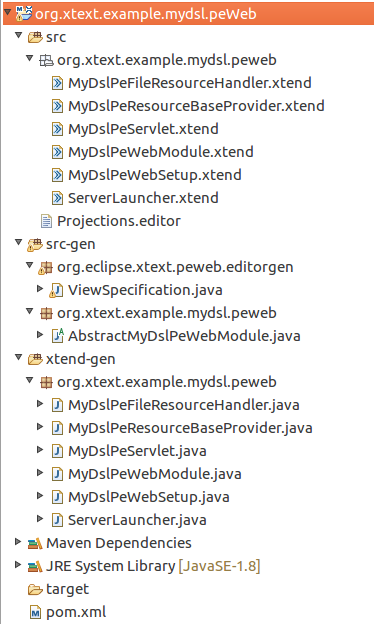
\includegraphics[width=0.4\linewidth]{./Screenshots/peWebProjectContentsAfterGeneration.png}
  \caption{The peweb project following generation}
  \label{fig:generatedPeWebProject}
\end{figure} \ref{fig:generatedPeWebProject}. Notice that MyDsl will be replaced with the name of the created language as specified when creating the project.
These files correspond to the following:
\begin{center}
\begin{tabular}{| m{7cm} | m{8cm} |}
\hline
File & Description \\
\hline \hline
Projections.editor & An empty file in which the language designer can specify the projections for the editor using the \emph{.editor} language discussed later.\\
\hline
MyDslPeServlet.xtend & A HTTP servlet which implements the projectional web API discussed later.\\
\hline
ServerLauncher.xtend & A servlet container to host MyDslPeWebServlet. When ran this starts the language server \\
\hline
MyDslPeFileResourceHandler.xtend & Allows the language designer to specify how files should be read or written, so that any persistence layer can be used. The generated file defaults to simply writing and reading files with the language's extension in the location given by  MyDslResourceBaseProvider \\
\hline
MyDslResourceBaseProvider.xtend & Used to specify how file URI's should be generated for a specified resource in the language. Defaults to a user-files folder at the location of the project.\\
\hline
MyDslPeWebModule.xtend & Allows binding of additional components in the language injector. This is where the resourceHandler and resourceBaseProviders are registered.\\
\hline
MyDslPeWebSetup.xtend & Creates the language injector itself, which will be used to inject information about the specified language into the otherwise generic language server implementation\\
\hline
\end{tabular}
\end{center}

All of the generated files, with the exception of the \emph{Projections.editor} and \emph{MyDslPeServlet}, are required by Xtext's default textual web integration, and so will be familiar to existing XText users. One thing of note is that the FileResourceHandler and ResourceBaseProvider files are not automatically generated in the textual case but are still required. Here by assuming a simple implementation of saving to the local file system, we can generate these files automatically and so enable language designers to get a language server running much more quickly in order to test their language. In fact, at this point, the language designer simply points the serverLauncher to the location of a client application to host, and the full web editor for their language is ready to run. There is no disadvantage to this generation as these files can be freely changed later or immediately.
\\
\\
%Maybe y generating like this at runtime we can use properties of the language. right now only name but could modify other things too.
%>Fact they are displayed to user means easily extensible matching requirement \RCustom
%>Talk about how the files generated are all commented (TODO) so clear what they are for and so easy to customise \RCustom

\printbibliography

\end{document}
